% !TEX root = ../main.tex

\chapter{Background} \label{chap:background}


\section{What is data science and why should we care?} \label{sec:data_science}
% data science vasta: gestione (data engineering) -> data exploration -> machine learning -> data viz



% DIKW pyramid
\todo{\begin{itemize}
\item{Data engineering}
\item{Data exploration}
\item{Machine learning and data understanding}
\item{Data visualization}
\end{itemize}}


\begin{itemize}
  \item cross-disciplinary field
  \item Drew Conway's Data Science Venn Diagram, first published on his blog in September 2010
  \item data-intensive applications (maybe)

\end{itemize}

\begin{figure}
  \centering
    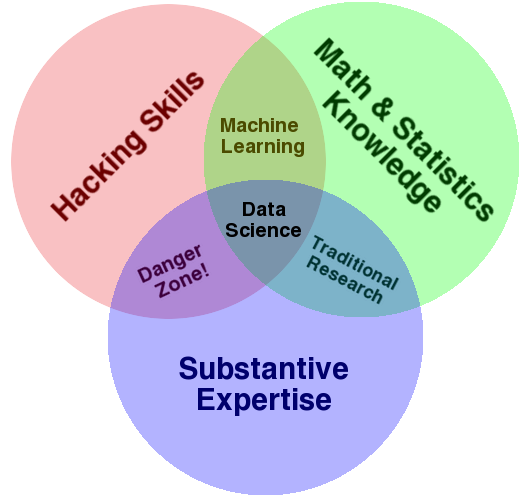
\includegraphics[width=0.5\textwidth]{part1/Data_Science_VD.png}
    \caption{Drew Conway's Data Science Venn Diagram\protect\footnotemark.} \label{fig:data_science_venn_diagram}
\end{figure}
 % BEWARE!! footnotetext is below at some point
 % FOOTNOTE text is here to prevent latex from putting it in weird places
 \footnotetext{\url{http://drewconway.com/zia/2013/3/26/the-data-science-venn-diagram}}

\section{Challenges in biomedical data science} \label{sec:challenges_biomedical}
% pochi sparsi rumorosi bucati
% this next section needs to be better rewritten
% Scientific progress has always been achieved by systematic observation of natural phenomena followed by experiments, measurements and consequently model formulation.
The process of modeling complex systems often implies collecting large amount of data in the field of life science, where large, multivariate and noisy measurements are typically acquired with the aim of describing multifactorial diseases.



In the era of personalized medicine, biospecimen collection and biological data management is still a challenging and expensive task~\cite{toga2015sharing}. Only few large-scale research enterprises, such as ENCODE~\cite{encode2004encode},  ADNI~\cite{jack2008alzheimer},  MOPED~\cite{kolker2012moped} or TCGA~\footnote{\url{https://cancergenome.nih.gov}}
, have sufficient financial and human resources to manage, share and distribute access of heterogeneous types of biological data. To date, many biomedical studies still rely on a small number of collected samples~\cite{mcneish2016effect, button2013power, yu2013shrinkage}. This effect is even worse in case of rare diseases~\cite{Garg2016ABM} or in high-throughput molecular data (\eg genomics and proteomics) where the dimensionality of the problem can be in the order of hundreds of thousands.
%
The setting where the number of measured variables heavily outnumbers the amount of collected samples is usually referred to as \textit{large p small n} scenario, or simply $n \ll p$. In this case, the main goal of the learning step is often to identify a meaningful subset of relevant variables that are the most representative of the observed phenomenon. In machine learning, this is known as variable/feature selection and several techniques addressing this task were presented so far~\cite{guyon2002gene}. Variable selection not only increases the prediction power of the learning machine, but it also promotes model interpretability, that is crucial in biology~\cite{altmann2010permutation}.
%
Regardless~\citep{okser2014regularized} of the learning machine, regularization can be introduced in several ways and it is of fundamental use in order to achieve the following desired properties:
%
\begin{itemize}
	\item identify models with good generalization properties, even with a limited amount of collected samples;
	\item achieve solutions that are robust to noise;
	\item learn the data structure when unknown;
	\item exploit prior knowledge on the data structure;
	\item promote interpretability performing variable selection;
	\item reduce the feasible set in order to help solving inverse problems. %\todo{this is for grown-ups :)}
\end{itemize}
%
%
% %when dealing with biological studies
In this paper we illustrate how regularization impacts in finding robust and meaningful models and we clarify how to choose the most suitable regularization scheme according to the biological context. The remainder of the paper is organized as follows: ....


\section{From clinical questions to data analysis} \label{sec:clinical_to_data}
In applied life science, the biological question at hand usually drives the data collection and therefore the statistical challenge to be solved. In order to achieve meaningful results, thorough data analysis protocol must be followed (see Section~\ref{subsec:model_selection}).
%\todo{XX Here we should say that if you do not follow rules in Section 5 all results may be meaningless}
In this section, my goal is to illustrate some of the most recurrent biological questions and how they can be translated into machine learning tasks.


\subsection{How to predict phenotypes from observed data?} % supervised learning
Starting from a collection of input measures that are likely to be related with some known target phenotype, the final goal here is to learn a model that represents the relationship between input and output. Several researches fall in this class, for instance in molecular (\eg lab tests, gene expression, proteomics, sequencing) \cite{angermueller2016deep, okser2014regularized, abraham2013performance} or radiomics/imaging studies (\eg MRI, PET/SPECT, microscopy) \cite{min2016deep, helmstaedter2013connectomic}. Biological questions of this class are usually tackled by \textit{supervised learning} models. In particular, when the observed clinical outcome is expressed as a one-dimensional continuous value, as in survival analysis, a \textit{single-output regression} problem is posed. Moreover, if the outcome is vector-valued, as in the case of multiple genetic trait prediction \cite{he2016novel}, the problem can be cast in a \textit{multiple-output regression }framework \cite{argyriou2008convex, baldassarre2012multi}. Biological studies involving categorical outcomes translate into \textit{classification} problems. In particular, if the clinical outcome assumes only two values, as in the \textit{case}-\textit{control} scenario, the classification problem is said to be \textit{binary}, whilst, if multiple classes are observed, the classification task becomes \textit{multi-class}.

\subsection{Which variables are the most significant?} % variable/feature selection
In the above case, a complementary question revolves around the interpretability of the predictive model. In particular, if dealing with high-throughput data, the main goal is to identify a relevant subset of meaningful variables for the observed phenomenon. This problem can be cast into a variable/feature selection problem \cite{guyon2002gene}. %To identify a model that uses only a reduced number of variables is of fundamental use in biology as it enhances its interpretability.
%\todo{group lasso for logistic regression- DNA sequences: \cite{}}

A machine learning model is said to be \textit{sparse} when it only contains a small number of non-zero parameters, with respect to the number of features that can be measured on the objects this model represents~\cite{hastie2015statistical, meier2008group}. This is closely related to feature selection: if these parameters are weights on the features of the model, then only the features with non-zero weights actually enter the model and can be considered \textit{selected}.

\subsection{How to stratify the data?} % clustering
Collecting measures from several samples, the final goal here is to divide them in homogeneous groups, according to some \textit{similarity} criterion. In machine learning, this is usually referred to as \textit{clustering}~\cite{hastie2009elements}.

\subsection{How to represent the samples?} % unsupervised feature learning and dimensionality reduction
In order to formulate a model of some natural phenomenon, it is necessary to design and follow a suitable data collection protocol. A natural question that may arise here is whether the raw collected measures are intrinsically representative of the target phenomenon or if some transformation must be applied in order to achieve a data representation that can be successfully exploited by a learning machine. For instance, it may be plausible to assume that the data lie in a low-dimensional embedding or that they can be better represented by a richer polynomial or Gaussian expansion.
A common solution, in this case, is to take advantage of \textit{feature engineering} techniques to obtain hand crafted features. However, this process can be very time-consuming and it may require the help of domain experts. The process of automatically identify suitable representations from the data itself is usually referred to as \textit{(un)supervised feature learning}~\cite{angermueller2016deep, mamoshina2016applications}.

\subsection{Are there recurring patterns in the data? } % \todo{maybe change title} sparse coding & dictionary learning
Analyzing data coming from complex domains, one may be interested in understanding whether complex observations can be represented by some combination of simpler events. In machine learning this typically translates into \textit{adaptive sparse coding} or \textit{dictionary learning} problems~\cite{masecchia2015genome, alexandrov2013signatures}.
%\todo{add bio example: pathological patterns in tumors from TCGA~\cite{alexandrov2013signatures},
%Neuroblastoma oncogenesis~\cite{masecchia2015genome}}


\subsection{How to deal with missing values?} % imputing
Applied life science studies must often deal with the issue of missing data. For instance, peaks can be missed in mass-spectrometry~\cite{jung2014adaption} or gene expression levels can be impossible to measure due to insufficient array resolution or image corruption~\cite{stekhoven2011missforest, troyanskaya2001missing}. Common strategies, such as discarding the samples with missing entries, or replacing the holes with the mean, median or most represented value, fall short when the missing value rate is high or the number of collected samples is relatively small. In machine learning this task usually translates into a \textit{matrix completion} problem~\cite{candes2009exact}.
